\chapter{Aplicación sobre datos}

\section{Cemento, análisis estructural y capacidades predictivas.}
\subsection*{Descripción del dataset}
\noindent El dataset  \cite{Yeh 2007} es un conjunto de datos recogidos de distintos tipos de cementos con distintas densidades, en particular tenemos las siguientes variables:
\begin{table}[h]
\footnotesize
\centering
\begin{tabular}{|l|l|l|l|}
\hline
Nombre & Tipo de dato & Medida & Descripción \\
\hline
Cemento (variable 1) & continuo & kg en una mezcla m3 & Variable predictora \\
Escoria de alto horno (variable 2) & continuo & kg en una mezcla m3 & Variable predictora \\
Ceniza volante (variable 3) & continuo & kg en una mezcla $m^3$ & Variable predictora \\
Agua (variable 4) & continuo & kg en una mezcla $m^3$ & Variable predictora \\
Superplastificante (variable 5) & continuo & kg en una mezcla $m^3$ & Variable predictora \\
Agregado grueso (variable 6) & continuo & kg en una mezcla $m^3$ & Variable predictora \\
Agregado fino (variable 7) & continuo & kg en una mezcla $m^3$ & Variable predictora \\
Edad & continuo & Día (1-365) & Variable predictora \\
Resistencia a la compresión & continuo & MPa & Variable respuesta \\
\hline
\end{tabular}
\end{table}

\noindent En total se recogen 1030 muestras de las cuales un 70\% se utilizan para el ajuste y un 30\% para construir una estimación del error cuadratico medio de predicción. 
\subsection*{Objetivos}

\noindent El estudio se divide en dos partes, una parte de análisis de la estructura de los datos mediante el análisis de componentes principales, en el que se busca ver cuales son las variables que mayor influencia tienen en la varianza del conjunto de datos tomados. 

\noindent Tras realizar este primer análsis exploratorio, se desarrollarán distintos modelos de regresión para comparar las capacidades predictivas. Los modelos a estudiar son un modelo lineal de regresión, un árbol de regresión y una red neuronal. 
\newpage
\subsection*{Desarrollo y resultados}

\noindent El análisis básico univariante de los datos arroja los siguientes datos:
\begin{figure}[h]
  \centering
  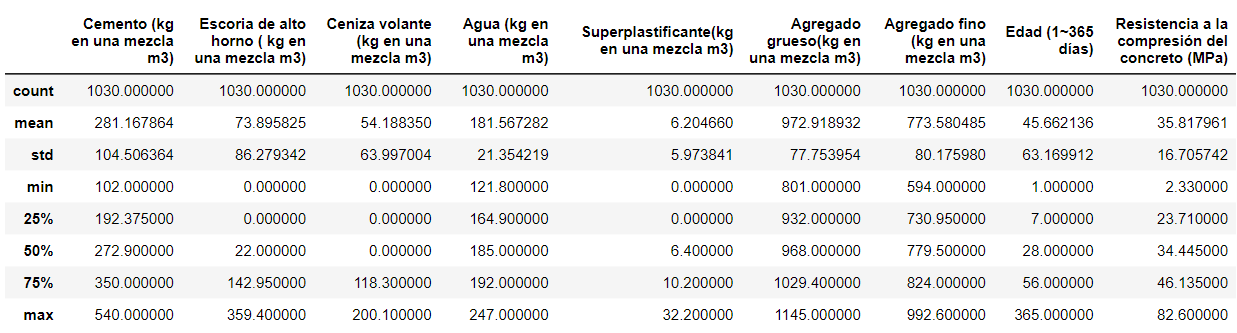
\includegraphics[scale=0.55]{Documentos Extra/Imagenes/Resumen_Basicos.png}
  \caption{Resumen univariante de los datos}
  \label{resumen_basicos}
\end{figure}


\noindent Ahora se calculan las componentes principales, estas se calculan con base en la matriz estandarizada. Tras aplicar dicho proceso, se obtienen el siguiente gráfico que representa las varianzas acumuladas:

\begin{figure}[h]
  \centering
  \includegraphics[scale=0.3]{Documentos Extra/Imagenes/Gráfico_varianza_explicada.png}
  \caption{Varianza acumulada frente al número de componentes principales}
  \label{ratio_varianzas}
\end{figure}

\noindent En particular, cuando tomamos las 3 primeras componentes principales estas representan un $62.5$\% de la variabilidad total, en particular esas componentes representan una variabilidad del  $25\%, 22\%, 16\%$ respectivamente. Y podremos llegar a a un $85\%$ si cogiésemos las 5 primeras. En nuestro caso, nos quedaremos con 3 para poder representar los datos en un espacio de dimensión reducida. 

\noindent Los coeficientes de las componentes principales obtenidos son los siguientes:
\begin{table}[ht]
\centering
\begin{tabular}{|l|c|c|c|}
\hline
&Componente 1& Componente 2& Componente 3\\\hline
Cemento  &0.04 & \textbf{0.54} & 0.36 \\ \hline
Escoria de alto horno &0.16 & 0.14 & \textbf{-0.70}\\ \hline
Ceniza volante &-0.37 & -0.27 & 0.02 \\ \hline
Agua&\textbf{0.56} & -0.12 & -0.12 \\ \hline
Superplastificante &\textbf{-0.54} & 0.25 & -0.19 \\ \hline
Agregado grueso &0.06 & -0.22 & \textbf{0.55} \\ \hline
Agregado fino& -0.38 & -0.19 & 0.00 \\ \hline
Edad &0.26 & 0.25 & 0.17 \\ \hline
Resistencia a la compresión &-0.11 & \textbf{0.63} & 0.03 \\ \hline
\emph{Variabilidad explicada} &0.25&0.22&0.12\\ \hline
\end{tabular} 
\end{table}

\noindent Añadir que al haber trabajado con la matriz de datos estandarizada, las coeficientes aquí mostrados son las correlaciones de cada una de las variables con la componente principal correspondiente. 

\noindent En el caso de la primera componente principal esta no tiene casi relación con la primera componente, mientras que la cantidad de \emph{Agua} y la cantidad de \emph{Superplastificante} influyen de manera notable. 

\noindent Por otro lado, la segunda componente está bastante correlada con la cantidad de \emph{Cemento} en la mezcla y con la \emph{Resistencia a la compresión}

\noindent Por último, es destacable que en este caso se elimina por completo la varible que mide la cantidad de \emph{Agregado fino}, mientras que la variable \emph{Escoria} influye de manera notable, aunque también es digna de mención la contribución de la cantidad de \emph{Agregado grueso}. 

\noindent A continuación, se presenta un gráfico el cual presenta los datos transformados por las 2 primeras componentes principales. 

\begin{figure}[h]
  \centering
  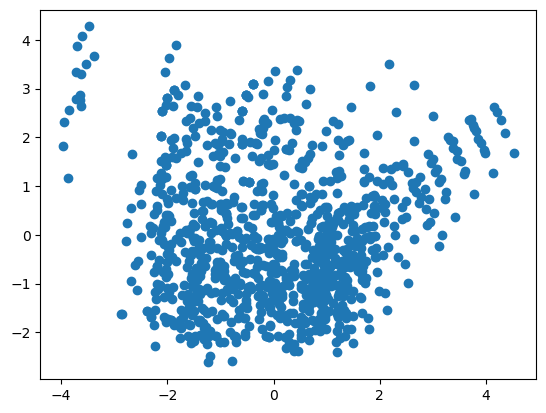
\includegraphics[scale=0.40]{Documentos Extra/Imagenes/PCA sobre Cemento.png}
  \caption{Datos representados en un espacio de dimensión 2.}
  \label{PCA en 2d}
\end{figure}

\noindent Se ajustan 3 modelos distintos, un modelo lineal, un árbol de regresión, y una red neuronal. 

\noindent Las características de los modelos y de los procesos de ajuste son los siguientes:

\noindent El modelo lineal es ajustado mediante el método de los minimos cuadrados obteniéndose un mínimo de error cuadrático de $106.14$ en el conjunto de entrenamiento mientras que en el conjunto de testeo se obtiene un error cuadrático medio de $108,21$. Además aunque no se pueda usar en el resto de modelos se obtiene en este caso un coeficiente de determinación $R^2$ de $0,62$ en el conjunto de ajuste. Por tanto, a nivel predictivo el modelo lineal tiene un buen rendimiento. 

\noindent El árbol de decisión utiliza el criterio CART de \emph{Breiman, L.}\cite{Breiman 1984}, ya que es el implementado por defecto en la librería \emph{Scikit-Learn} de Python. Este modelo proporciona un error cuadrático medio de  $108.22$ sobre el conjunto de ajuste mientras que sobre el conjunto de testeo proporciona un error cuadrático de $57.55$, lo que implica que tiene una buena capacidad predictiva. 

\noindent En la red neuronal se ha elegido un modelo simple con dos capas, la primera con 13 neuronas con una función de activación lineal rectificada, en cambio, la otra capa contiene únicamente una neurona con una función lineal. En este caso el ajuste de la red neuronal obtiene un error cuadrático medio de $MSE=46.56$ en el ajuste y un $MSE=47.54$ en el conjunto de prueba, en principio, tenemos un modelo que comete menos error en el conjunto de prueba. 

\noindent Hay que destacar que ninguno de los modelos ha incurrido en problemas de sobreajuste, es decir, no se ha tenido casos en los que el valor del error medio en el conjunto de ajuste sea mucho menor que en el conjunto de prueba. 

\noindent Una vez ajustados los modelos, se pueden tomar los valores predichos para los datos de prueba y graficarlos frente a los valores reales, en cada caso tendremos los puntos en azul y la recta roja representaría los puntos los cuales su predicción es igual al valor real. 

\begin{figure}[ht]
  \centering
  \begin{minipage}{0.32\textwidth}
   
    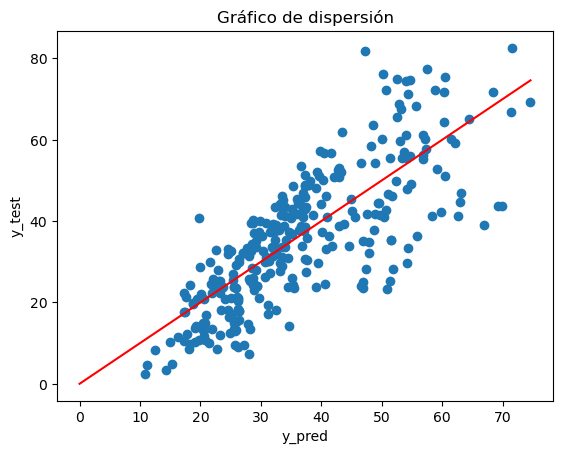
\includegraphics[width=\textwidth]{Documentos Extra/Imagenes/Datos PruebasRegresionLineal.png}
    \caption{Regresión Lineal}
    \label{fig:regresion_lineal}
  \end{minipage}
  \hfill
  \begin{minipage}{0.32\textwidth}
  
    \includegraphics[width=\textwidth]{Documentos Extra/Imagenes/Datos PruebasÁrbolesRegresion.png}
    \caption{Árbol de Regresión}
    \label{fig:regression_tree}
  \end{minipage}
  \begin{minipage}{0.33\textwidth}
    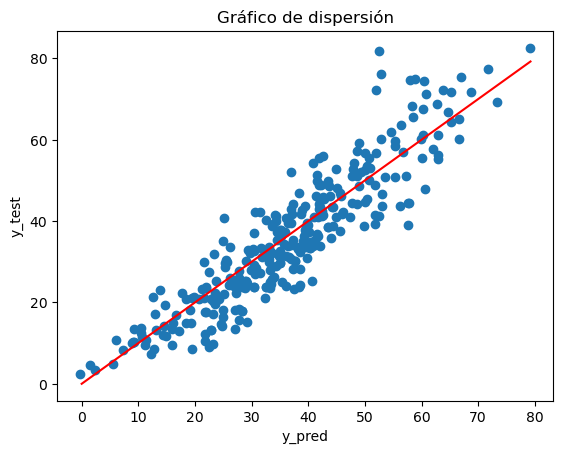
\includegraphics[width=\textwidth]{Documentos Extra/Imagenes/Datos PruebasRedNeuronal.png}
    \caption{Red Neuronal}
    \label{fig:red_neuronal}
  \end{minipage}
 \end{figure}

\noindent Se puede ver que en el caso del modelo lineal \ref{fig:regresion_lineal} los puntos son más lejanos de la recta. Por tanto, tenemos que el primer caso en principio tendrá peores predicciones.

\noindent En resumen, obtenemos los siguientes resultados:

\begin{table}[ht]
\centering
\begin{tabular}{|l|c|c|c|}
\hline
 & Modelo Lineal & Árbol de Regresión &  Red Neuronal \\
\hline
Conjunto Ajuste &  $106.14$  &  $108.22$& $46.56$\\
Conjunto de Prueba & $108,21$   & $57.55$ &  $47.54$ \\
\hline
\end{tabular}
\caption{Errores cuadráticos medios en cada conjunto}
\label{tab:tabla_ejemplo}
\end{table}


\subsection*{Conclusiones}
\noindent En conclusión, podemos concluir que el modelo lineal no es la mejor opción para realizar predicciones. Aún así este tipo de modelos son útiles para sacar otro tipos de conclusiones como por ejemplo influencias lineales con la variable independiente. 

\noindent En cambio, los modelos de árbol de regresión y la red neuronal proporcionan mejores predicciones de manera altamente significativa con relación a la regresión mediante un modelo lineal. En contraste, las redes neuronales no otorgan la sencillez en la interpretación que tienen los modelos lineales, además permiten seguir trabajando más allá de la predicción, cosa que no pasa con las redes neuronales.  

\noindent Por otro lado, la sensibilidad a los cambios de los datos de ajuste que sufren los árboles los hace una opción peor a la hora de utilizar uno solo, problema solucionado por \emph{Breiman, L.}\cite{Breiman 1996,Breiman 2001}, pero se pierden las carácteristicas beneficiosas del árbol de decisión. 